% \pagebreak[4]
% \hspace*{1cm}
% \pagebreak[4]
% \hspace*{1cm}
% \pagebreak[4]

\chapter{Cơ sở lý thuyết} \label{theory-basis}

\ifpdf
    \graphicspath{{TheoryBasis/Chapter1Figs/PNG/}{TheoryBasis/Chapter1Figs/PDF/}{TheoryBasis/Chapter1Figs/}}
\else
    \graphicspath{{TheoryBasis/Chapter1Figs/EPS/}{TheoryBasis/Chapter1Figs/}}
\fi

Trong nội dung của chương này, đồ án sẽ trình bày về các kiến thức cơ bản cũng như như các thuật toán được sử dụng trong hệ thống tư vấn.
\section{Khảo sát các hệ tư vấn đã có}

Hệ thống tư vấn đã trở thành một đề tài khá phổ biến trong khoảng thời gian gần đây. Trong lĩnh vực xây dựng các hệ thống tư vấn trong quá khứ, người ta đã làm việc và nghiên cứu khá nhiều và ứng dụng rộng rãi trên các lĩnh vực khác nhau. Hầu hết công việc chủ yếu tập trung phát triền những phương pháp gợi ý những những đối tượng ưa thích đến cho người dùng. Ví dụ như những trang web gợi ý những bộ phim, gợi ý những quyển sách mà người dùng có thể yêu thích. Hệ thống tư vấn thông thường sẽ tiếp cận và giải quyết vấn đề theo 1 trong 2 hướng: Lọc dựa trên nội dung ( \textit{content-based filtering}) hoặc lọc cộng tác (\textit{collaborative filtering}). Tuy nhiên trên thực tế, việc áp dụng cả 2 hướng để giải quyết vấn đề cũng thường được cân nhắc trong việc giải quyết bài toán trong thực tế. (\textit{hybrid recommender system})

\subsection{Lọc cộng tác} là phương pháp được xây dựng dựa trên lý thuyết : "Những người có cùng hứng thú/mong muốn/sở thích về một vấn đề gì đó trong quá khứ thì có thể họ sẽ cũng có cùng hứng thú/mong muốn/sở thích trong tương lai". Ví dụ: hai người dùng A và B có chung sở thích ăn uống, họ đã mua các đồ ăn giống nhau. Nếu B còn thích thêm cả Cocacola nữa thì rất có thể A cũng thích, nên ta có thể gợi ý cho A mua thêm Cocacola. 

Phương pháp này thực hiện việc thu thập và đánh giá một lượng lớn thông tin về hành vi, sở thích của người dùng để tiên đoán sở thích của họ dựa trên sự giống nhau về thông tin giữa các người dùng. Ưu điểm của phương pháp này là nó không phải phụ thuộc vào việc nhận định, đánh giá để “hiểu được” nội dung của đối tượng tư vấn mà vẫn có thể đưa ra được kết quả thoả mãn mong muốn của người dùng. Tuy nhiên mặt hạn chế của phương pháp trên là nó cần một lượng lớn dữ liệu nguời dùng đa dạng để có thể hoạt động chính xác được. Và việc tính toán hành vi của từng người dùng cũng tiêu hao một lượng lớn tài nguyên máy tính.

\subsection{Lọc dựa trên nội dụng} là phương pháp mà người ta quân tâm đến 2 thực thể chính là người dùng và đối tượng được khuyến nghị đến cho người dùng. Quá trình lọc thực hiện bắt đầu từ việc xây dựng một hồ sơ người dùng (user profile) là tập các ưu tiên về sở thích của người dùng về đối tượng, và hồ sơ miêu tả đối tượng. Sau đó tiến hành lọc kết quả dựa vào phương pháp context-matching. Đây là phương pháp bắt nguồn từ lĩnh vực nghiên cứu triết xuất thông tin và lọc thông tin.

Hệ thống tư vấn trong tài liệu này áp dụng phương pháp lọc dựa trên nội dung, và cân nhắc thêm lọc cộng tác khi hệ thống đã phát triển sau này.

\section{Thuật toán Context-matching}
Thuật toán context-matching sử dụng để giải quyết bài toán cần Context-matching với Partial-matching ( khi mà khả năng đạt được “perfect match” là thấp ). Xây dựng các input context, output context và hàm đánh giá giữa các properties của chúng. Mục tiêu cuối cùng là một giá trị Boolean thể hiện sự phù hợp, hay không phù hợp của thực thể được tính đến.\\

Mô hình thuật toán được biểu diễn ở hình sau : 

\begin{figure}[!htbp]
  \begin{center}
    %\leavevmode
    \ifpdf
      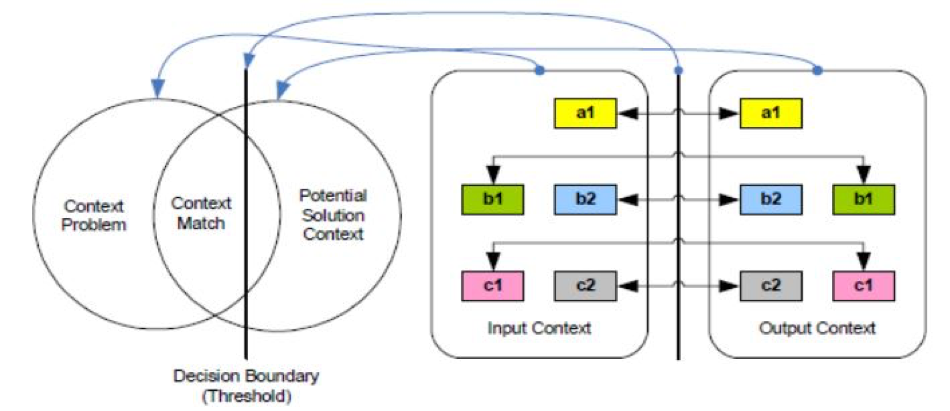
\includegraphics[scale=1]{contextmatch}
    \else
      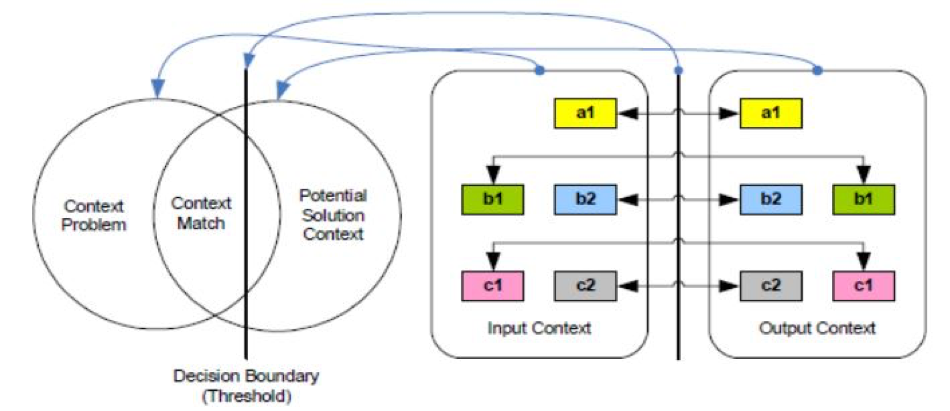
\includegraphics[scale=1]{contextmatch}
    \fi
    \caption{Mô hình thuật toán Context Matching }
    \label{ContextMatching}
  \end{center}
\end{figure}
\subsection{Tổng quan}	
Cấu trúc cơ bản của thuật toán là ${ON <event> IF <condition> THEN <action>}$. Trong đó $<event>$ có thể là context data cần tính (event khởi động), hoặc là kết quả trả về của một lần so sánh ở phía trên, $<condition>$ là cách so sánh giữa một input context property với một output context property sẽ được báo cáo dưới đây, $<action>$ là kết quả của việc đánh giá trên $<condition>$ và nó có thể là việc tiếp tục so sánh input và output tiếp theo hoặc là giá trị Boolean quyết định độ phù hợp của context (action cuối cùng).
\subsection{Input context và output context }	
Input context là nguyên mẫu để so sánh, các kết quả phù hợp là những kết quả phải có độ match với input context lớn nhất định. Output context là giải pháp tiềm năng cho vấn đề cần giải quyết trong bài toán, là một số lượng những thực thể đem so sánh với input context, được trích xuất từ cấu trúc dữ liệu. Từ input và output context, cần xây dựng một bộ các context properties là những thuộc tính bên trong quyết định context. Việc so sánh sẽ là so sánh giữa các context property.
\subsection{Các giá trị sử dụng}	
Giả sử áp dụng thuật toán cho bộ context properties $[a1, b1, b2, c1, c2]$. Ta có : 
\begin{itemize}
\item $w$: giá trị trong khoảng $[0.10...1.00]$ phản ánh mức độ ưu tiên của thuộc tính 
\item $e$:  giá trị đánh giá xem thuộc tính ở input và output có match nhau không, $e$ được biểu diễn trong khoảng $[0...1]$
\item $av = (e * w)$ :  giá trị thực tế đánh giá độ match của thuộc tính, nằm trong khoảng  $[0.00...1.00]$
\item $sav = av(a_1) + av(b_1) + av(b_2) + av(c_1) + av(c_2)$ : tổng giá trị $av$ 
\item $mpv$: giá trị sav cao nhất có thể đạt được. Nó thể hiện trường hợp mà tất cả các context property đều match nhau. 
\item $rv = \dfrac{sav}{mpv}$ : giá trị trả về sau so sánh. Nó đánh giá tổng quan xem kết quả context match đến mức độ nào, nằm trong khoảng $[0.00...1.00]$.  
\item $t$: giá trị cho ngưỡng đạt $[0.10...1.00]$. Context match  phù hợp khi so sánh ta có giá trị $rv > t$. 
 \end{itemize}
\subsection{Các bước thực hiện thuật toán }	
 \begin{itemize}
\item Bước 1: Đánh giá context match cho từng context property -> rút ra giá trị $e$ . 
\item Bước 2: Thiết lập giá trị $w$ đã được định sẵn cho từng context property
\item Bước 3: Tính giá trị $av$ của thuộc tính $av = (e* w)$
\item Bước 4: Tính tổng các giá trị $av$ của cả quá trình đánh giá $sav = av(a_1) + av(b_1) + av(b_2) + av(c_1) + av(c_2)$
\item Bước 5: Tính giá trị $sav$ cao nhất có thể đạt $mpv = w(a_1) + w(b_1) +w(b_2) + w(c_1) + w(c_2)$
\item Bước 6: Tính giá trị kết quả trả về $rv = \dfrac{sav}{mpv}$
\item Bước 7: Sử dụng giá trị ngưỡng đã có sẵn để xác định xem output context có match với input context hay không . IF $(rv) >= (t)$ THEN $context-match = true$ [1] or IF $(rv) < (t)$ THEN $context-match = false$ [0]
 \end{itemize}
\section{Kỹ thuật Kansei Engineering}

\subsection{Tổng quan}

Kansei Engineering là kỹ thuật tích hợp khía cạnh cảm xúc của con người vào trong quá trình xây dựng sản phẩm, nhằm mục đích tạo ra được sản phẩm phù hợp với yêu cầu và mong muốn của người dùng. Nó là việc mang lại sự hài lòng, thoả mãn cho người dùng một cách có khoa học. Để đạt được điều đó, trải nghiệm của người dùng dựa trên các sản phẩm tương tự được thu thập và phân tích, từ đó thiết lập mô hình dự đoán mối quan hệ giữa cảm xúc của con người và các đặc tính vật lý của sản phẩm.

3 điểm chính được chú trọng trong Kansei Engineering đó là :
\begin{itemize}
	\item Làm thế nào để hiểu được cảm xúc nội tâm của người dùng
	\item Làm thế nào để phản ánh hiểu biết đó vào trong việc phát triển sản phẩm
	\item Làm thế nào để xây dựng một hệ thống có tổ chức theo định hướng Kansei Engineering
\end{itemize}

\subsection{Mô hình}
Mặc dù nhiều mô hình Kansei Engineering khác nhau phục vụ cho các bài toán cụ thể khác nhau. Nhưng về cơ bản, tất cả đều tuân theo mô hình tổng quát \cite{KE05} sau đây:
\begin{figure}[H]
  \begin{center}
    %\leavevmode
    \ifpdf
      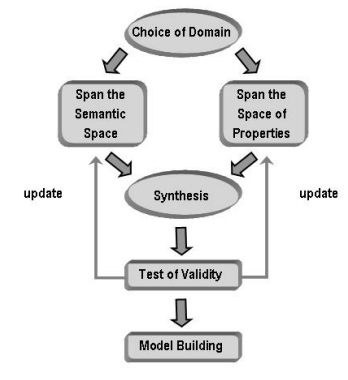
\includegraphics[scale=0.9]{kanseimodel}
    \else
      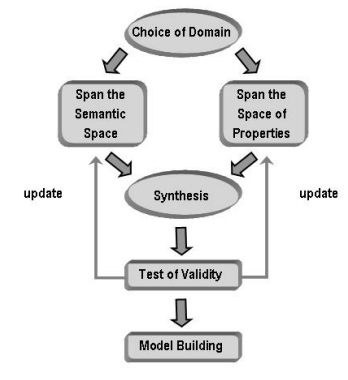
\includegraphics[scale=0.9]{kanseimodel}
    \fi
    \caption{Mô hình tổng quát Kansei Engineering}
    \label{KanseiModel}
  \end{center}
\end{figure}

\textbf{Chọn miền chủ đề}\\

Chủ đề mang ý nghĩa là ý tưởng tổng quát đằng sau sản phẩm. việc lựa chọn miền chủ đề trong đó bao gồm lựa chọn loại sản phẩm sẽ xét đến, đối tượng người dùng sử dụng và các đặc tả cụ thể khác. Tiếp theo đó, miền không gian Kansei và miền không gian thuộc tính sản phẩm sẽ được xác định. Chúng sẽ được phân tích trong bước tổng hợp để tìm ra mối quan hệ giữa thuộc tính của sản phẩm và cảm xúc của người dùng. Từ đó xác định được thuộc tính sản phẩm sẽ ảnh hưởng đến người dùng như thế nào.\\

\textbf{Mở rộng miền không gian Kansei}\\

Osgood et al\cite{osgood} đề xuất rằng mọi vật đều có thể được miêu tả bằng miền không gian vector cảm xúc. Từ miền chủ đề đã xác định, các từ khoá Kansei Word sẽ được thu thập. Kansei Word là các danh từ, tính từ cảm xúc mà người dùng có thể sử dụng để miêu tả về sản phẩm. Số lượng từ khoá thu thập được sẽ đa dạng tuỳ theo từng loại chủ đề khác nhau, giao động từ 100 đến 1000 từ khoá khác nhau. Tuy nhiên, do yếu tố chủ quan của con người, một số từ khoá có thể mang ý nghĩa tương đồng hoặc gần giống nhau. Do vậy tập từ khoá này sau đó sẽ được nhóm lại với nhau bằng phương pháp thủ công hoặc toán học. cuối cùng, chúng phân tích để chọn ra được những từ khoá đại diện mang ý nghĩa tổng quát độc lập với nhau.

\begin{figure}[H]
  \begin{center}
    %\leavevmode
    \ifpdf
      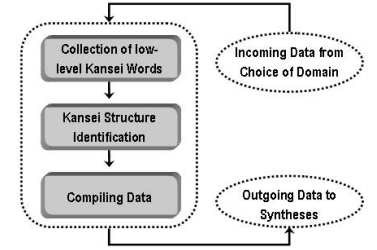
\includegraphics[scale=0.9]{semanticspan}
    \else
      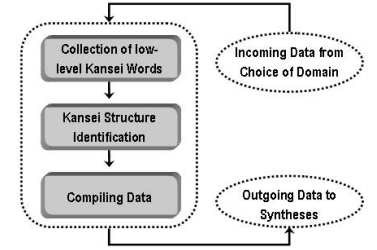
\includegraphics[scale=0.9]{semanticspan}
    \fi
    \caption{Quy trình mở rộng miền không gian Kansei}
    \label{SemanticSpanningPhase}
  \end{center}
\end{figure}

\textbf{Mở rộng miền không gian thuộc tính sản phẩm}\\

Tương tự như bước Mở rộng miền không gian Kansei, ở bước này, các thuộc tính của sản phẩm như hình thức, màu sắc, thể loại, nội dung..v..v... được thu thập từ các sản phẩm khác. Các sản phẩm được chọn để khai thác thuộc tính có thể là các sản phẩm đang lưu hành trên thị trường, đề xuất của khách hàng, hoặc thậm chí là ý tưởng thiết kế mới. Tương tự, do có thể có sự tương đồng giữa các thuộc tính gây ảnh hưởng đến độ chính xác  nên các thuộc tính được chọn ra là các thuộc tính tiêu biểu nhất của sản phẩm.\\

\textbf{Tổng hợp}\\

Trong bước tổng hợp, 2 miền không gian từ khoá Kansei và thuộc tính sản phẩm sẽ được móc nối vào với nhau. Mỗi từ khoá Kansei Word sẽ tương ứng với một hoặc nhiều thuộc tính của sản phẩm, ảnh hưởng trực tiếp đến các thuộc tính đó. Như trong nghiên cứu về thiết kế lon bia của Ishihara et al. (1998)\cite{ishihira98} cho thấy rằng, cảm giác "đắng" của người uống chịu ảnh hưởng bởi màu sắc và hình dạng logo lon bia, với màu đen và logo vuông cho người uống cảm giác "rất đắng", trong khi màu trắng và logo hình bầu dục tạo cảm giác ngược lại.

 \begin{figure}[H]
  \begin{center}
    %\leavevmode
    \ifpdf
      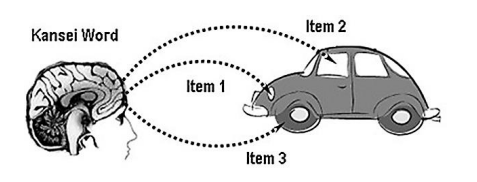
\includegraphics[scale=0.9]{kanseisynthesis}
    \else
      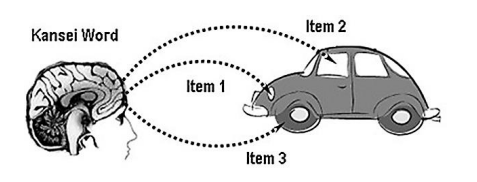
\includegraphics[scale=0.9]{kanseisynthesis}
    \fi
    \caption{Pha tổng hợp}
    \label{KanseiSynthesis}
  \end{center}
\end{figure}

Có nhiều phương pháp tổng hợp, trong đó phổ biến là:
\begin{itemize}
	\item Category Identification
	\item Regression Analysis/Quantification Theory Type I
	\item Rough Sets Theory
	\item Genetic Algorithm
	\item Fuzzy Sets Theory\\
\end{itemize}  

\textbf{Kiểm tra độ chính xác}\\

Trước khi mô hình đã xây dựng có thể đem vào sử dụng. Nó cần được phải được kiểm tra độ chính xác, đánh giá xem nó có đủ độ tin cậy và phù hợp với thực tế hay không. Trong trường hợp mô hình không đạt yêu cầu, cần có sự thay đổi trong các bước trên rồi tiếp tục quy trình đánh giá lại cho đến khi ra được kết quả đạt yêu cầu cuối cùng.	

\section{Computerized Adaptive Testing}

\subsection{Tổng quan}
Computerized Adaptive Testing - Bài thi tương tác tuỳ biến qua máy tính là hình thức làm bài thi trên máy tính. Trong đó, nội dung và độ khó của câu hỏi sẽ được tuỳ chỉnh sao cho phù hợp với năng lực của thí sinh dự thi. Sau mỗi câu hỏi, trình độ của thí sinh được cập nhập, quyết định độ khó của câu hỏi tiếp theo. Nếu thí sinh trả lời tốt các câu hỏi trước đó, hệ thống sẽ đưa ra các câu hỏi có độ khó cao hơn. Ngược lại, nếu thí sinh trả lời sai nhiều, độ khó của câu hỏi tiếp theo sẽ được giảm xuống. Và khi đến một ngưỡng nhất định, đã xác định chắc chắn được trình độ của thí sinh thì bài kiểm tra sẽ được hoàn tất.\\

 \begin{figure}[H]
  \begin{center}
    %\leavevmode
    \ifpdf
      \includegraphics[scale=0.5]{cat}
    \else
      \includegraphics[scale=0.5]{cat}
    \fi
    \caption{Computerized Adaptive Test}
    \label{ComputerizeAdaptiveTest}
  \end{center}
\end{figure}

\subsection{Mô hình}
Mô hình CAT cơ bản gồm 4 bước sau đây:
\begin{itemize}
	\item Chọn ra câu hỏi từ tập câu hỏi dựa vào trình độ thí sinh
	\item Câu hỏi được chọn sẽ được thí sinh trả lời, đúng hoặc sai
	\item Trình độ của thí sinh sẽ được cập nhập, dựa vào kết quả của tất cả những câu hỏi đã trả lời
	\item Lặp lại quá trình trên cho đến khi một ngưỡng quy định trước đạt được.
\end{itemize} 

\subsection{Ưu điểm}
Với phương thức khác hoàn toàn với bài kiểm tra trên giấy thông thường, với CAT mỗi thí sinh được nhận các bài thi hoàn toàn khác nhau. Hơn nữa, số lượng câu hỏi thí sinh cần phải trả lời sẽ được giảm thiểu. Thí sinh sẽ không phải trả lời những câu hỏi quá khó so cũng như quá dễ so với trình độ của họ, do đó thời gian làm bài trung bình sẽ ngắn hơn so với bài kiểm tra thông thường song vẫn cho ra kết quả chính xác tương tự.

\section{Các cơ sở lý thuyết về công nghệ sử dụng}
\subsection{Firebase}
Firebase là một dịch vụ cơ sở dữ liệu thời gian thực hoạt động trên nền tảng đám mây được cung cấp bởi Google nhằm giúp các lập trình phát triển nhanh các ứng dụng bằng cách đơn giản hóa các thao tác với cơ sở dữ liệu.

Firebase hỗ trợ tối đa đối với những ứng dụng Backend, nó bao gồm các tiện ích lưu trữ dữ liệu, xác thực người dùng, static, hosting,… Vì thế giúp cho lập trình viên giảm thiểu công việc, và tập trung nâng cao trải nghiệm người dùng.\\

\textbf{Realtime Database – Cơ sở dữ liệu thời gian thực}
 
Firebase lưu trữ dữ liệu database dưới dạng JSON và thực hiện đồng bộ database tới tất cả các client theo thời gian thực. Cụ thể hơn là bạn có thể xây dựng được client đa nền tảng (cross-platform client) và tất cả các client này sẽ cùng sử dụng chung 1 database đến từ Firebase và có thể tự động cập nhật mỗi khi dữ liệu trong database được thêm mới hoặc sửa đổi.
 
 \begin{figure}[!htbp]
  \begin{center}
    %\leavevmode
    \ifpdf
      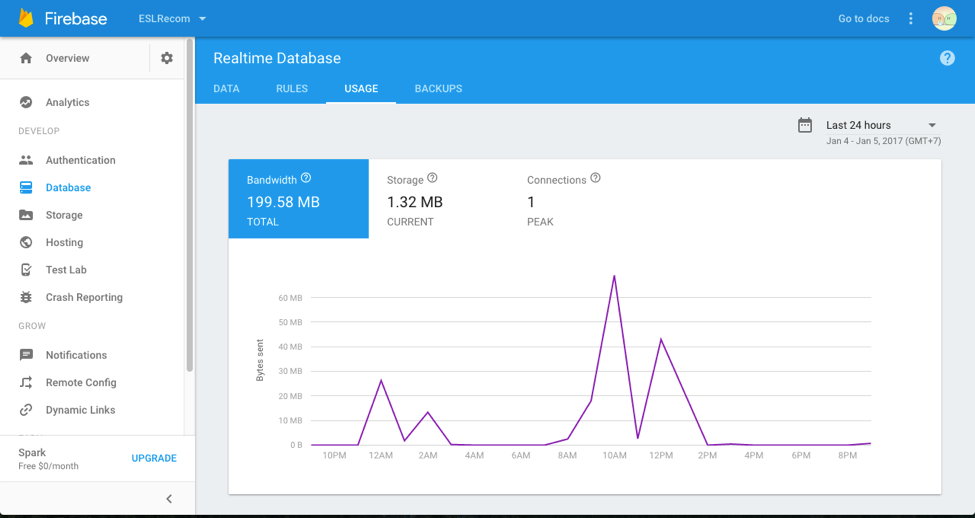
\includegraphics[scale=0.9]{firebasedb}
    \else
      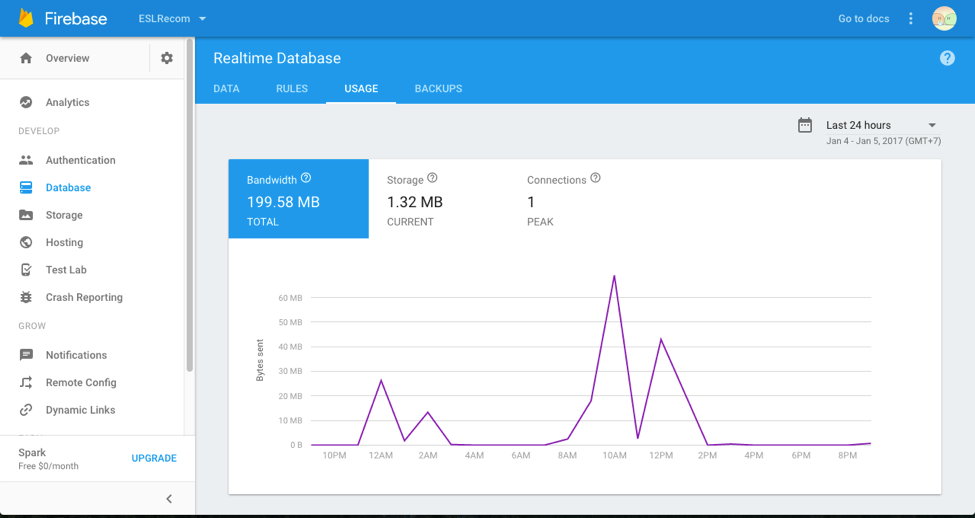
\includegraphics[scale=0.9]{firebasedb}
    \fi
    \caption{Cơ sở dữ liệu thời gian thực }
    \label{FirebaseDB}
  \end{center}
\end{figure}

 \begin{figure}[!htbp]
  \begin{center}
    %\leavevmode
    \ifpdf
      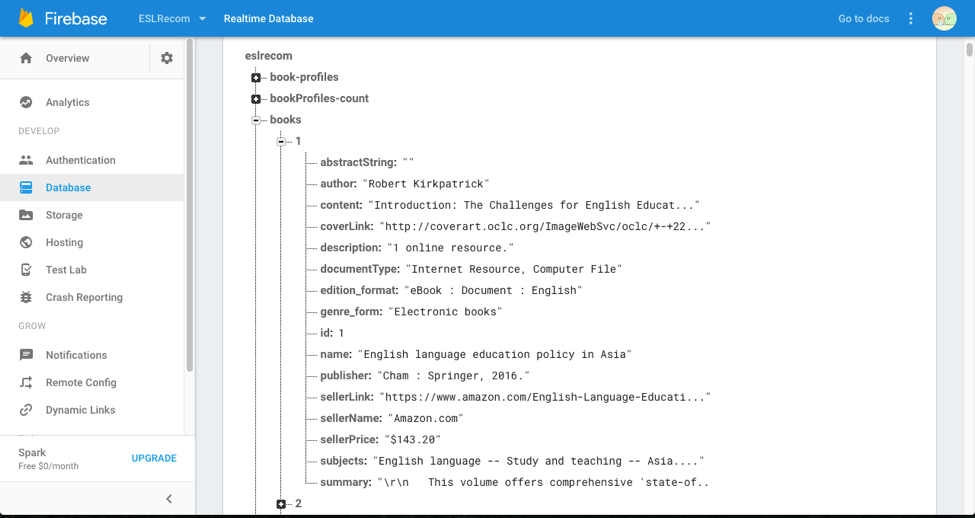
\includegraphics[scale=0.9]{firebasedb2}
    \else
      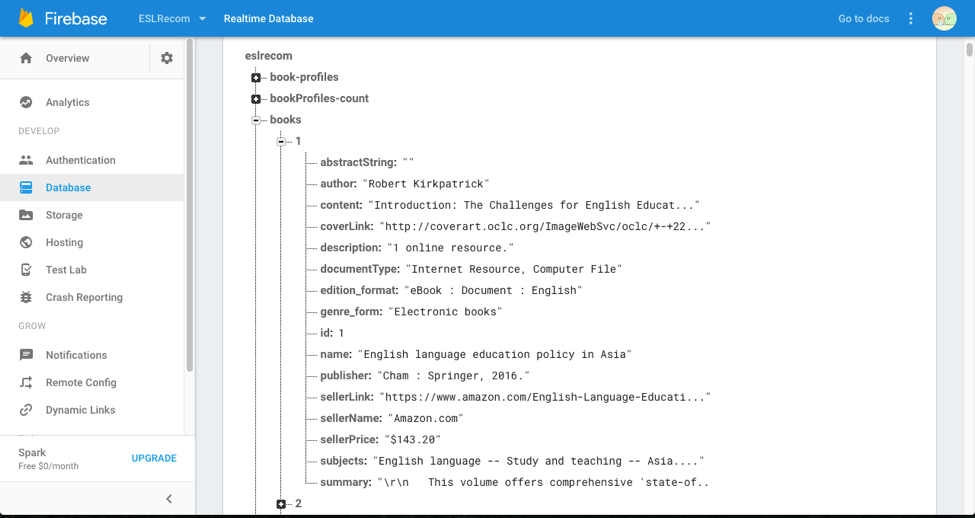
\includegraphics[scale=0.9]{firebasedb2}
    \fi
    \caption{Lưu trữ cơ sở tri thức chia sẻ giữa các thiết bị}
    \label{FirebaseDB2}
  \end{center}
\end{figure}

\subsection{Scrapy}

Scrapy là một framework được viết bằng Python, nó cấp sẵn 1 cấu trúc tương đối hoàn chỉnh để thực hiện việc crawl và extract data từ website một cách nhanh chóng và dễ dàng. Bạn muốn lấy dữ liệu từ các website nhưng dữ liệu đó quá lớn để copy rồi paste vào database của bạn, scrapy hỗ trợ bạn làm điều đó. Việc lấy dữ liệu website hoàn toàn tự động nhanh chóng và việc sử dụng scrapy cũng rất đơn giản giúp bạn tiếp kiệm được nhiều thời gian và công sức.

 \begin{figure}[!htbp]
  \begin{center}
    %\leavevmode
    \ifpdf
      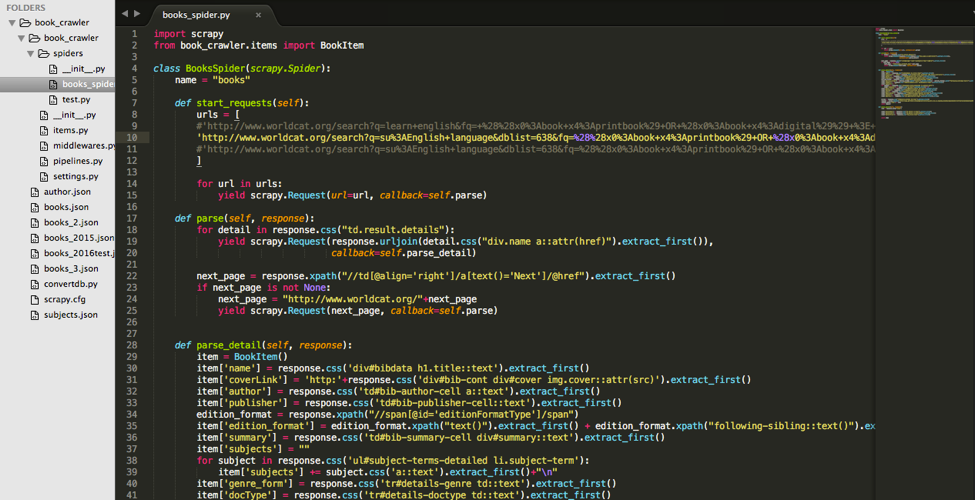
\includegraphics[scale=0.9]{scrapy}
    \else
      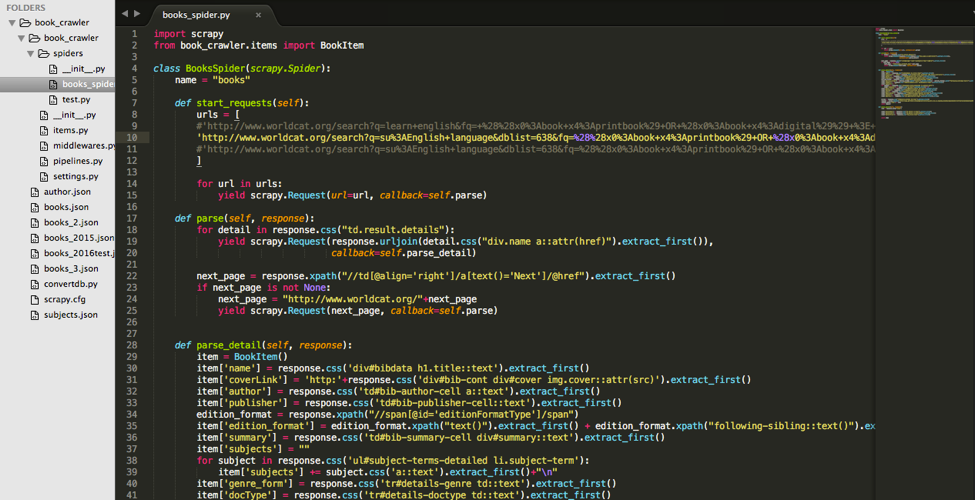
\includegraphics[scale=0.9]{scrapy}
    \fi
    \caption{Crawl tài liệu từ thư viện điện tử WorldCat.org }
    \label{Scrapy}
  \end{center}
\end{figure}

\subsection{Thuật toán $tf-idf$}

Viết tắt của thuật ngữ tiếng Anh term frequency – inverse document frequency,$tf-idf$ là thuật toán dùng để tìm trọng số của một từ trong văn bản thu được qua thống kê thể hiện mức độ quan trọng của từ này trong một văn bản, mà bản thân văn bản đang xét nằm trong một tập hợp các văn bản.

Nguyên lý cơ bản của $tf-idf$ là "độ quan trọng của một từ sẽ tăng lên cùng với số lần xuất hiện của nó trong văn bản và sẽ giảm xuống nếu như từ đó xuất hiện trong nhiều văn bản khác". Do đó trọng số của một từ $t$ trong tài liệu $f$ sẽ được tính bằng $tf * idf$, với $tf$ là độ phổ biến của từ $t$ trong tài liệu $f$ và $idf$ là nghịch đảo độ phổ biến của từ $t$ trong các tài liệu còn lại của tập tài liệu. Cụ thể theo công thức sau đây:

\begin{equation}
tf(t, d) * idf(t, D) = \dfrac{f_d(t)}{\max_{w \in d} f_d(w)} * \log{\dfrac{|D|}{|d \in D : t \in d|}}\\\\\\
\end{equation}

Lấy ví dụ một văn bản chứa 100 từ, trong đó từ "cat" xuất hiện 3 lần. Giá trị $tf$ của "cat" sẽ là   $\dfrac{3}{100} = 0.03$. Tiếp theo, giả dụ có 10 triệu văn bản và từ "cat" xuất hiện ở 1000 văn bản trong đó. Giá trị $idf$ sẽ là $\log{\dfrac{10,000,000}{1,000}} = 4$. Vậy trọng số $tf-idf$ của từ khoá "cat" sẽ là $0.03 * 4 = 0.12$.
